\documentclass[a4paper]{oblivoir}
\usepackage{amsmath,amssymb,kotex,kswrapfig,mdframed,paralist}
\usepackage{fapapersize}
\usefapapersize{210mm,297mm,20mm,*,20mm,*}

\usepackage{tabto,pifont}
\TabPositions{0.2\textwidth,0.4\textwidth,0.6\textwidth,0.8\textwidth}
\newcommand\tabb[5]{\par\noindent
\ding{172}\:{\ensuremath{#1}}
\tab\ding{173}\:\:{\ensuremath{#2}}
\tab\ding{174}\:\:{\ensuremath{#3}}
\tab\ding{175}\:\:{\ensuremath{#4}}
\tab\ding{176}\:\:{\ensuremath{#5}}}

\usepackage{graphicx}

\pagestyle{empty}

%%% Counters
\newcounter{num}

%%% Commands
\newcommand\prob[1]
{\bigskip\par\noindent\stepcounter{num} \textbf{문제 \thenum) #1}\par\noindent}

\newcommand\pb[1]{\ensuremath{\fbox{\phantom{#1}}}}

\newcommand\ba{\ensuremath{\:|\:}}

\newcommand\vs[1]{\vspace{25pt}}

\newcommand\an[1]{\bigskip\par\noindent\textbf{문제 #1)}\par\noindent}

%%% Meta Commands
\let\oldsection\section
\renewcommand\section{\clearpage\oldsection}

\let\emph\textsf

\begin{document}
\begin{center}
\LARGE준영, 미니테스트 14
\end{center}
\begin{flushright}
날짜 : 2017년 \(\pb3\)월 \(\pb{10}\)일 \(\pb{월}\)요일
,\qquad
제한시간 : \pb{17년}분
,\qquad
점수 : \pb{20} / \pb{20}
\end{flushright}

%
\prob{}
\begin{minipage}{0.45\textwidth}
함수 \(y=f(x)\)의 그래프가 오른쪽 그래프와 같을 때, 다음 <보기>중 옳은 것을 골라라.
\end{minipage}
\begin{minipage}{0.45\textwidth}\centering
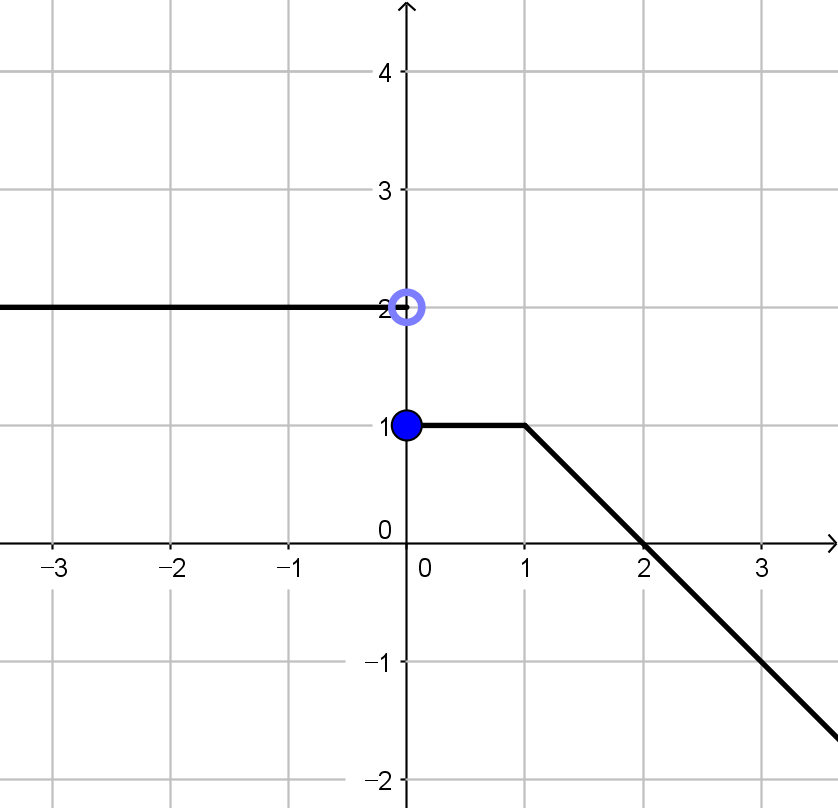
\includegraphics[width=0.45\textwidth]{continuity_test}
\end{minipage}

\begin{mdframed}[frametitle=<보기>]
\begin{enumerate}
\item[ㄱ.]
\(f(x)\)는 두 곳에서 불연속이다.
\item[ㄴ.]
\(f(x)\)는 두 곳에서 미분 불가능하다.
\item[ㄷ.]
\(f(x)\)는 \(x=1\)에서 미분가능하다.
\item[ㄹ.]
\(xf(x)\)는 \(x=0\)에서 미분가능하다.
\item[ㅁ.]
\(x^2f(x)\)는 \(x=0\)에서 미분가능하다.
\end{enumerate}
\end{mdframed}

%
\prob{}
함수 
\(f(x)=\begin{cases}
x^2+1	&(x\ge1)\\
ax+b	&(x<1)
\end{cases}\)
가 실수 전체에서 미분가능할 때, 상수 \(a\), \(b\)의 값을 각각 구하여라.

%
\prob{}\label{type1}
다음 두 과정을 따라 포물선 \(y=x^2+4x+2\) 위의 점 \((1,7)\)에서의 접선의 방정식을 구하여라.

\noindent\fbox{과정1 : 수학1에서의 방법}
\begin{enumerate}[(1)]
\item
이 접선의 기울기를 \(m\)이라고 할 때, 이 접선 \(l\)은 기울기가 \(m\)이고 \((1,7)\)를 지나는 직선이므로
\begin{align*}
l:y&=m(x-\pb1)+\pb7\\
&=\pb mx+\pb{-m+7}
\end{align*}
\item
직선 \(l\)과 포물선이 접하므로, 직선 \(l\)과 포물선은 \pb{1}개의 점에서 만난다.
그러므로 다음 연립방정식
\[
\begin{cases}
y=x^2+4x+2\\
y=\pb mx+\pb{-m+7}
\end{cases}
\]
은 \pb{1}개의 근을 가진다.
연립방정식을 풀어보면,
\[x^2+4x+2=\pb mx+\pb{-m+7}\]
\[x^2+\pb{(-m+4)}x+\pb{(m-5)}=0\]
\item
이 이차방정식이 중근을 가져야 한다.
따라서 \(D=0\)이다.
\begin{align*}
D=\pb{(-m+4)}^2-4\pb{(m-5)}=0\\
m^2-\pb{12}m+36=0\\
m=\pb6
\end{align*}
\item
따라서 구하는 접선 \(l\)의 방정식은
\[l:y=\pb6x+1\]
\end{enumerate}

\noindent\fbox{과정2 : 미적분1에서의 방법}
\begin{enumerate}[(1)]
\item
\(f(x)\)를 \(f(x)=x^2+4x+2\)라고 하자.
도함수인 \(f'(x)\)를 계산하면
\[f'(x)=\pb{2x+4}\]
\item
\(y=f(x)\) 위의 점 \((1,f(1))\)에서의 기울기는 \(f'(1)\)인데 이것을 계산하면
\[f'(1)=\pb6\]
\item
따라서 접선 \(l\)은 \((\pb1,\pb7)\)을 지나고 기울기가 \pb6인 직선이다;
\begin{align*}
l:y&=\pb6(x-\pb1)+\pb7\\
l:y&=6x+\pb1
\end{align*}
\end{enumerate}

%
\prob{}\label{type2}
다음 두 과정을 따라 기울기가 \(2\)인 포물선 \(y=x^2+4x+2\)의 접선의 방정식을 구하여라.

\noindent\fbox{과정1 : 수학1에서의 방법}
\begin{enumerate}[(1)]
\item
이 접선의 \(y\)절편을 \(n\)이라고 하면, 이 접선 \(l\)은 기울기가 \(2\)이고 \(y\)절편이 \(n\)인 직선이므로
\[y=2x+n\]
로 놓을 수 있다.
\item
직선 \(l\)과 포물선이 접하므로, 직선 \(l\)과 포물선은 \pb{1}개의 점에서 만난다.
그러므로 다음 연립방정식
\[
\begin{cases}
y=x^2+4x+2\\
y=2x+n
\end{cases}
\]
은 \pb{1}개의 근을 가진다.
연립방정식을 풀어보면,
\[x^2+4x+2=2x+n\]
\[x^2+\pb2x+\pb{(2-n)}=0\]
\item
이 이차방정식이 중근을 가져야 한다.
따라서 \(D=0\)이다.
\begin{align*}
D=\pb2^2-4\pb{(2-n)}=0\\
n=\pb1
\end{align*}
\item
따라서 구하는 접선 \(l\)의 방정식은
\[l:y=\pb2x+1\]
\end{enumerate}

\noindent\fbox{과정2 : 미적분1에서의 방법}
\begin{enumerate}[(1)]
\item
\(f(x)\)를 \(f(x)=x^2+4x+2\)라고 하자.
도함수인 \(f'(x)\)를 계산하면
\[f'(x)=\pb{2x+4}\]
\item
이 접선의 접점을 \((t,f(t))\)라고 하면, 이 접선의 기울기는 \(f'(t)\)이다.
이것이 \(\pb{2}\)와 같아야 하므로
\[f'(t)=\pb2\]
\[2t+4=2\]
\[t=-1\]
\item
따라서 접선 \(l\)은 \((\pb1,\pb7)\)을 지나고 기울기가 \pb6인 직선이다;
\begin{align*}
l:y&=\pb6(x-\pb1)+\pb7\\
l:y&=2x+\pb1
\end{align*}
\end{enumerate}

%
\prob{}\label{type3}
다음 두 과정을 따라 포물선 \(y=x^2+4x+2\) 밖의 한 점 \((0,1)\)에서 그은 접선의 방정식을 모두 구하여라.

\noindent\fbox{과정1 : 수학1에서의 방법}
\begin{enumerate}[(1)]
\item
이 접선의 기울기를 \(m\)이라고 할 때, 이 접선 \(l\)은 기울기가 \(m\)이고 \((0,1)\)를 지나는 직선이므로
\begin{align*}
l:y&=m(x-\pb0)+\pb1\\
&=\pb mx+\pb{1}
\end{align*}
\item
직선 \(l\)과 포물선이 접하므로, 직선 \(l\)과 포물선은 \pb{1}개의 점에서 만난다.
그러므로 다음 연립방정식
\[
\begin{cases}
y=x^2+4x+2\\
y=\pb mx+\pb{1}
\end{cases}
\]
은 \pb{1}개의 근을 가진다.
연립방정식을 풀어보면,
\[x^2+4x+2=\pb mx+\pb{1}\]
\[x^2+\pb{(-m+4)}x+\pb{1}=0\]
\item
이 이차방정식이 중근을 가져야 한다.
따라서 \(D=0\)이다.
\begin{align*}
D=\pb{(-m+4)}^2-4\pb{1}=0\\
m^2-\pb{8}m+12=0\\
m=\pb2,\qquad m=\pb6
\end{align*}
\item
따라서 구하는 접선은 \(\pb2\)이고, 이 접선들을 각각 \(l_1\), \(l_2\)라고 하면
\[l_1:y=2x+\pb{1},\qquad l_2:y=6x+\pb1\]
\end{enumerate}

\noindent\fbox{과정2 : 미적분1에서의 방법}
\begin{enumerate}[(1)]
\item
\(f(x)\)를 \(f(x)=x^2+4x+2\)라고 하자.
도함수인 \(f'(x)\)를 계산하면
\[f'(x)=\pb{2x+4}\]
\item
이 접선의 접점을 \((t,f(t))\)라고 하면, 이 접선은 \((t,f(t))\)를 지나고 기울기가 \(f'(t)\)인 직선이다.
따라서
\[l:y=f'(t)(x-t)+f(t)\]
\[l:y=\pb{2t+4}(x-t)+\pb{\(t^2+4t+2\)}\tag{\(\ast\)}\]
이다.
이 직선이 \((0,1)\)을 지나야 하므로
\[\pb{1}=\pb{2t+4}(\pb{0}-t)+\pb{\(t^2+4t+2\)}\]
\[t^2=\pb1\]
\[t=\pb{-1},\qquad t=\pb1\]
\item
\(t=\pb{-1}\)일 때의 직선을 \(l_1\), \(t=1\)일 때의 직선을 \(l_2\)라고 하면, \((\ast)\)로부터
\end{enumerate}
\begin{minipage}{0.45\textwidth}
\begin{align*}
l_1:y&=\pb2(x-\pb{-1})+\pb{-1}\\
l_1:y&=\pb2x+1
\end{align*}
\end{minipage}
\begin{minipage}{0.45\textwidth}
\begin{align*}
l_1:y&=\pb6(x-\pb{1})+\pb7\\
l_1:y&=\pb6x+1
\end{align*}
\end{minipage}

\begin{minipage}{0.45\textwidth}
%
\prob{}
문제 3--5에서의 접선들과 \(y=x^2+4x+2\)의 그래프룰 오른쪽 모눈에 모두 그리시오.








\end{minipage}
\begin{minipage}{0.45\textwidth}
\par\bigskip\includegraphics[width=0.9\textwidth]{55}
\end{minipage}
\end{document}